\documentclass[usenames,dvipsnames]{beamer} 

\usepackage[orientation=portrait,scale=1.5,size=a1]{beamerposter} 
\usepackage{svg}
\usepackage{tcolorbox}
\usepackage{background}
\usepackage{lipsum}  
\usepackage{tgheros}
   
\usebackgroundtemplate{\includesvg[height=\paperheight]{template}}%
\setbeamercolor{title}{fg=white} 
\setbeamercolor{author}{fg=white} 
\setbeamercolor{institute}{fg=white} 
\setbeamercolor{date}{fg=red}  
 
 % Poster title
\title{\Huge \textbf{The NeXus Constructor}} 
\subtitle{\Large Visualising the Configuration of Neutron Experiments with Qt for Python}
\author{\large \textbf{Jack Harper\inst{1}}, \textbf{Dolica Akello-Egwel\inst{1}}, Matthew Jones\inst{1,}\inst{2}, Dominic Oram\inst{1}, Jonas Nilsson\inst{3}, Tobias Richter\inst{3} }
\institute{\normalsize   
\inst{1} ISIS Facility, Rutherford Appleton Laboratory, Didcot, Oxfordshire, UK  \,\, 
\inst{2} Tessella Ltd., Abingdon, Oxfordshire, UK
\inst{3} European Spallation Source, Lund, Sweden
}

% Remove Date
\date{}

% Remove Beamer Navigation Symbols
\setbeamercolor*{frametitle}{bg=}
\setbeamertemplate{navigation symbols}{}

\begin{document}
\begin{frame}[t]
  
\maketitle

\begin{columns}[t]  
\begin{column}{0.47\paperwidth}

%%%%%%%%%%% Start of Column 1 %%%%%%%%%%
\begin{tcolorbox}[colback=white,colframe=white,title=Introduction,coltitle=blue]
\bigskip
Accelerator experiments would be pointless without data analysis and visualisation. In order to perform accurate data analysis, you need to lay out where each component is with high precision, such as neutron detectors, which capture the pulse of energy after going through a sample, or disk choppers, which cut the beam of neutrons up.

\end{tcolorbox}

\bigskip

\begin{tcolorbox}[colback=white,colframe=white,title=Scientific Facilities and the NeXus Standard,coltitle=blue]
\bigskip


NeXus is an effort by an international group of scientists to define a common data exchange and archival format for neutron, X-ray and muon experiments. NeXus is built on top of the scientific data format HDF5 and adds domain-specific rules for organizing data within HDF5 files, in addition to a dictionary of well defined domain-specific field names. The NeXus data format has two purposes. First, it defines a format that can serve as a container for all relevant data associated with a beamline. This is a very important use case. Second, it defines standards in the form of application definitions for the exchange of data between applications. NeXus provides structures for raw experimental data as well as for processed data.

\bigskip
A recent addition to the NeXus standard means components that are used in experiments can specify shape definition to describe their placement, size and geometry. Transformations (NXtransformations) can be applied to these components when their position changes during or before the experiment. 

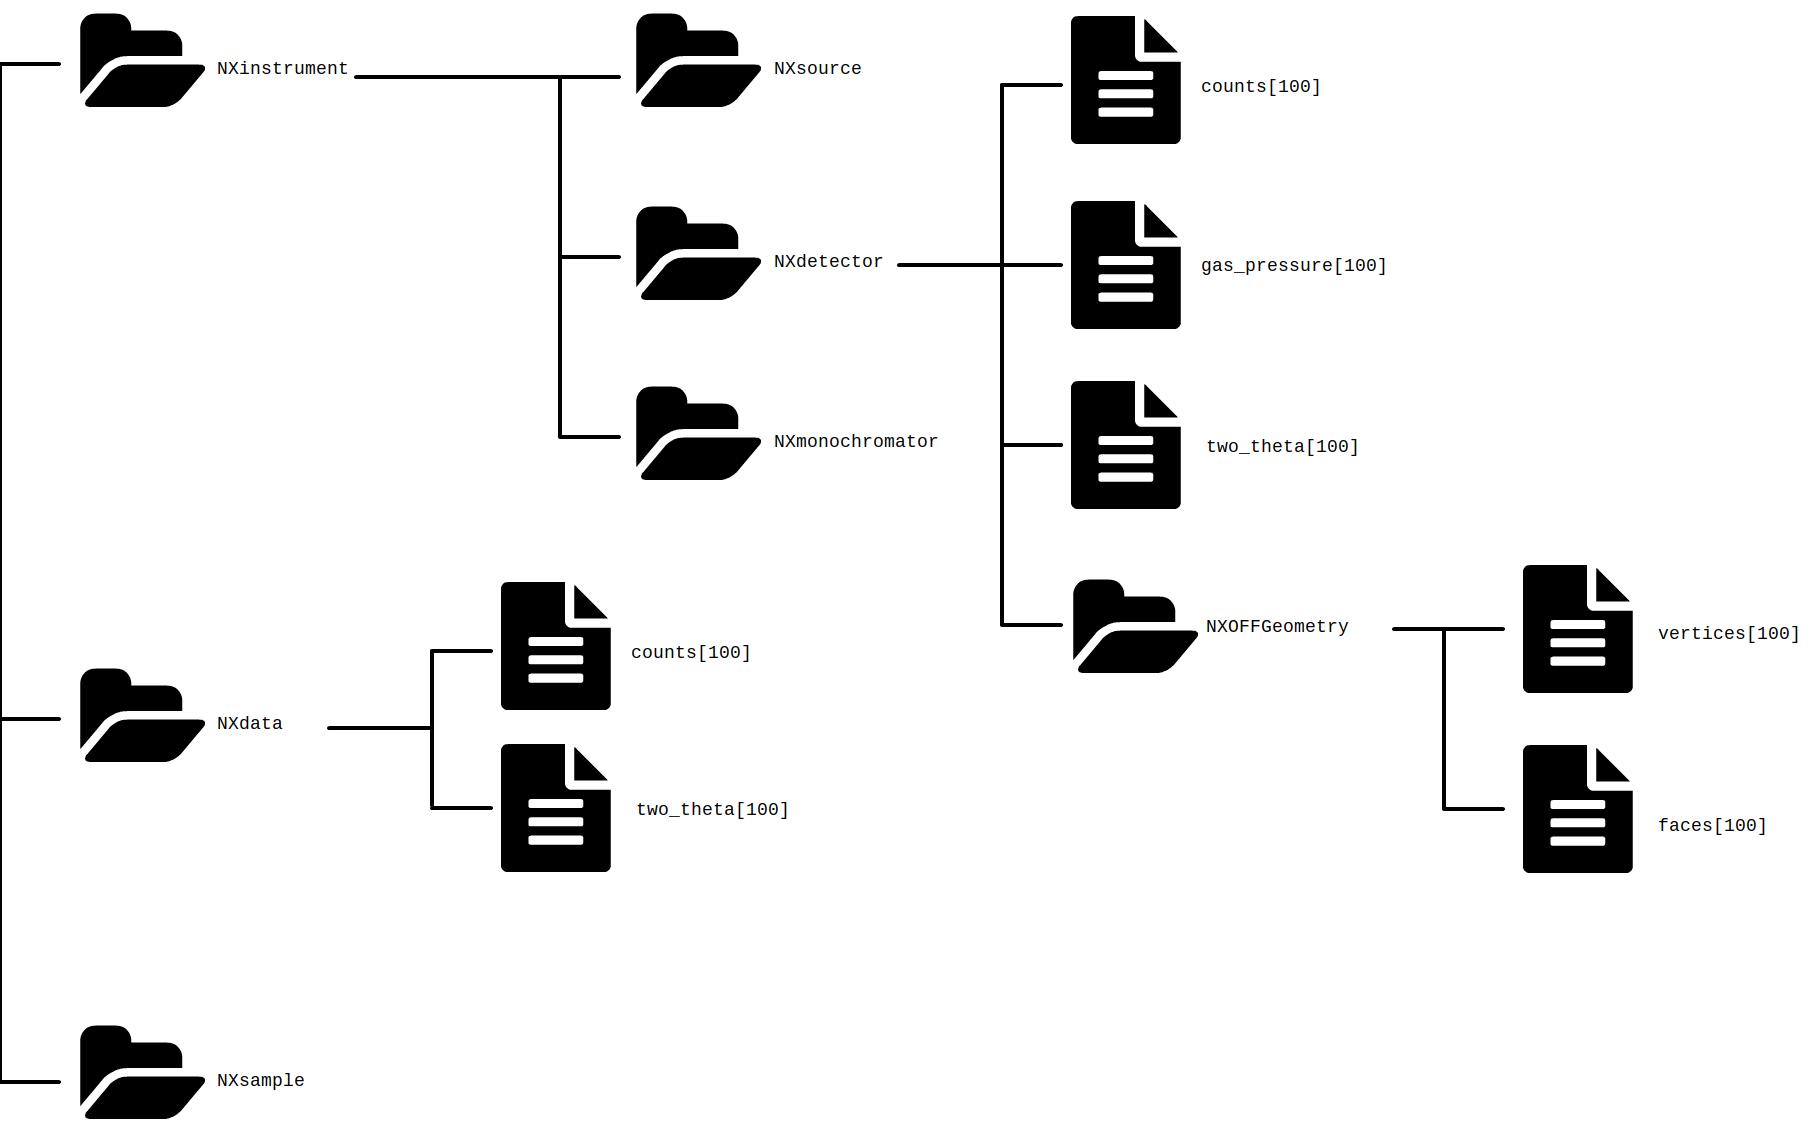
\includegraphics[width=\linewidth]{nexusdiagram.png}


Currently, there is no tool for visualising and editing NeXus files. The section below describes our solution for this and how we are implementing a tool containing this functionality. NeXus files are outputted by the experiment, and tools need to be configured to write them. This is currently being done manually by editing large JSON files which is both fragile and time-consuming. 

\end{tcolorbox}

\bigskip

\begin{tcolorbox}[colback=white,colframe=white,title=The NeXus Constructor,coltitle=blue]
\bigskip
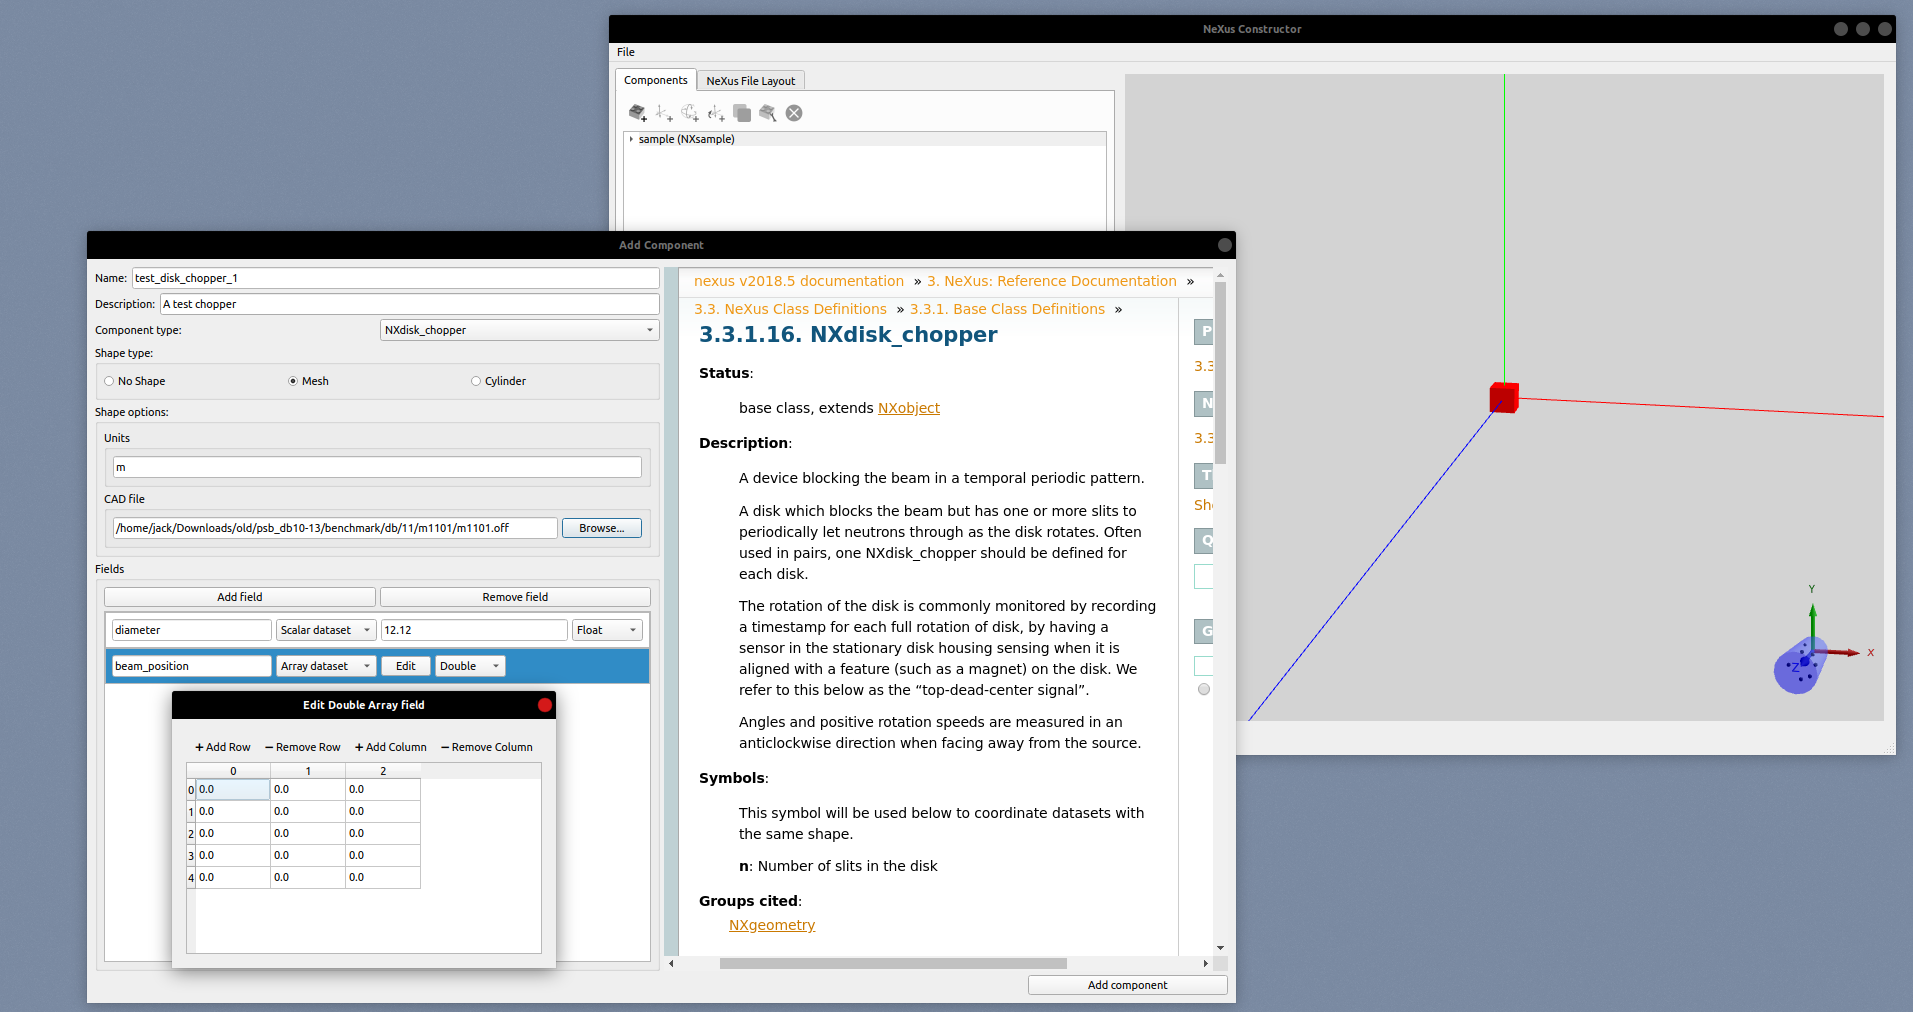
\includegraphics[width=\linewidth]{screenshot.png}



\lipsum[2]
\end{tcolorbox}

\end{column}   
%%%%%%%%%% End of Column 1 %%%%%%%%%%

%%%%%%%%%% Start of Column 2 %%%%%%%%%%
\begin{column}{0.47\paperwidth}  

\begin{tcolorbox}[colback=white,colframe=white,title=Qt for Python,coltitle=blue]
\bigskip
We are using Qt for Python(PySide2) for the NeXus Constructor's graphical user interface. These are the official bindings for Qt 5 C++ API, provided by the Qt company. 
\bigskip

There are two main methods of using Qt in Python, the more common "Widgets" framework or Qt-Quick which uses a markup language called QML.
We are taking the Qt-Widgets approach to developing the NeXus constructor, as the tooling for Qt-Quick/QML seems to be a bit lacking and some of the bindings are not pythonic, and rather use C++-like idioms. Widgets also look more native to the OS running them. 
\bigskip

Since version 5.12 PySide2 has included the Qt3D module in Qt5. We are utilising this with our 3d View of components in the neutron experiments. Qt3D provides a high-level interface to OpenGL which allows us to display the geometry information of components as well as an animated pulsed neutron beam.
\bigskip
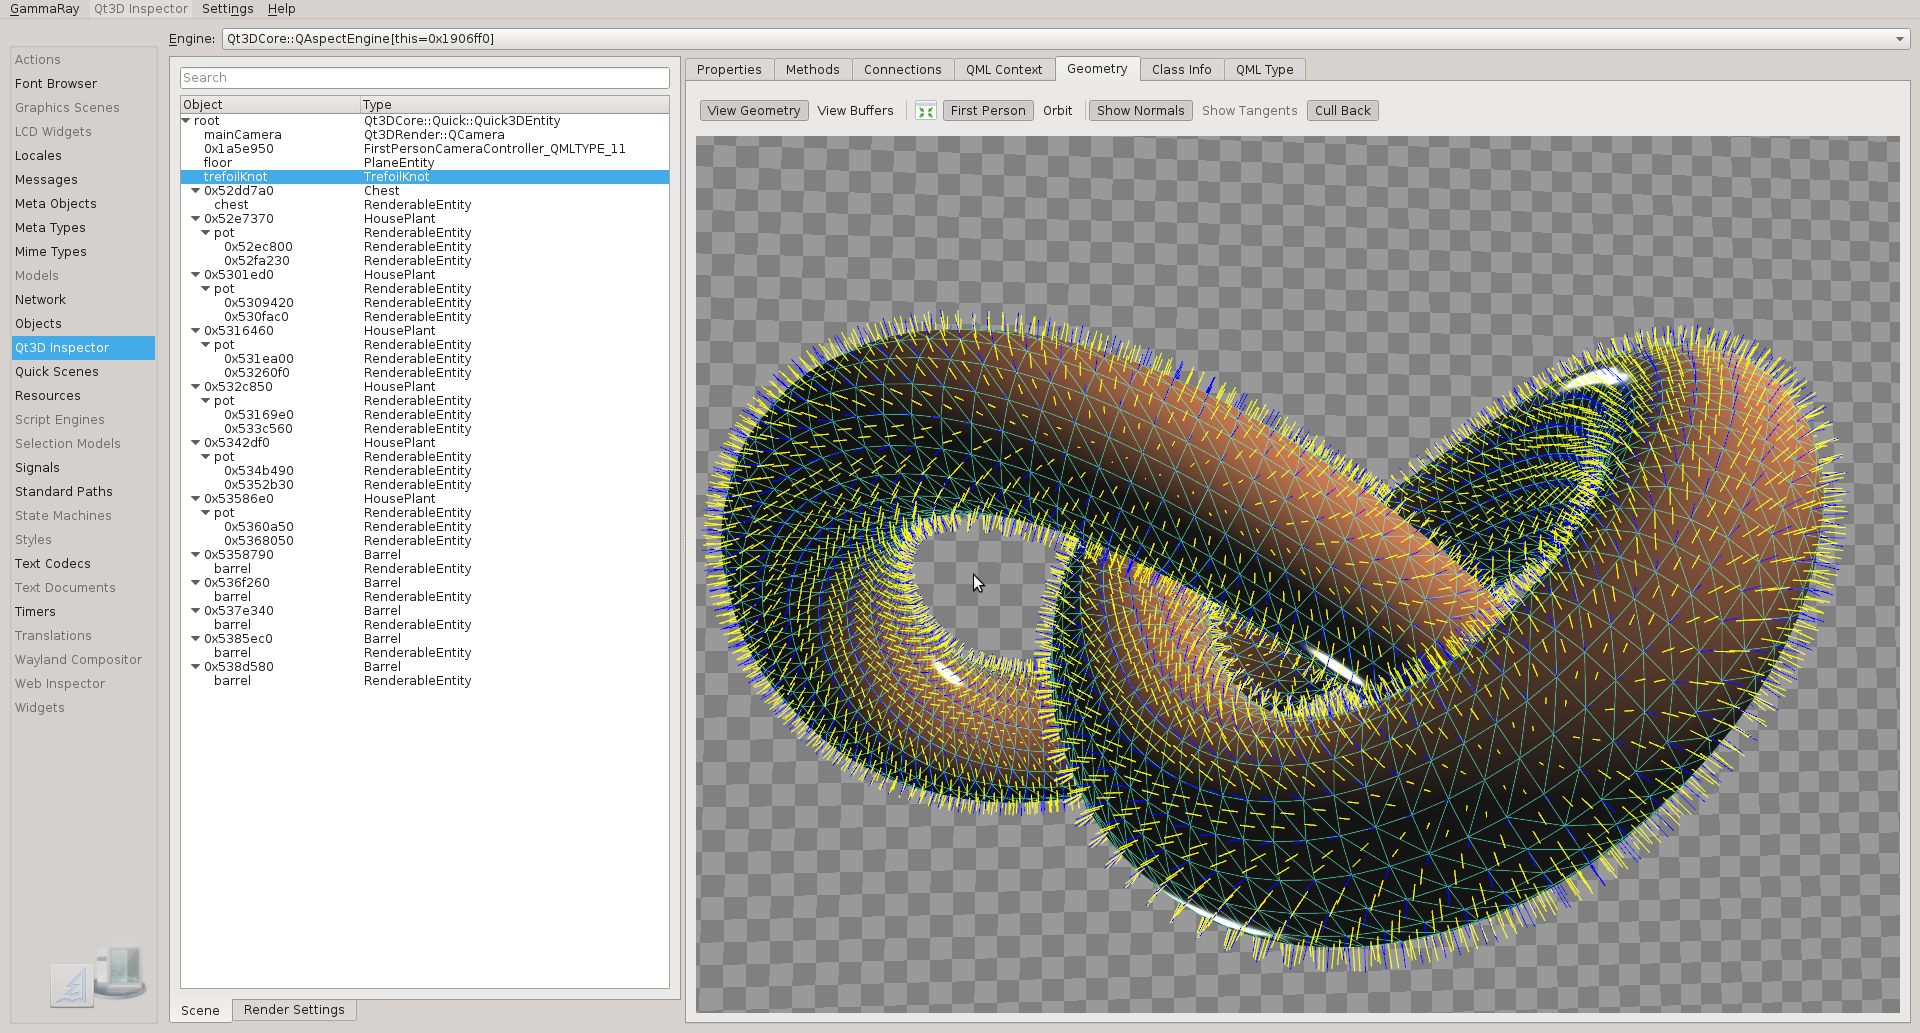
\includegraphics[width=\linewidth]{qt3d.png}
\bigskip


\end{tcolorbox}

\bigskip


\bigskip

\begin{tcolorbox}[colback=white,colframe=white,title=Conclusion,coltitle=blue]
\lipsum[2]
\end{tcolorbox}

\end{column}
%%%%%%%%%% End of Column 2 %%%%%%%%%%  
\end{columns}
 
\end{frame}
\end{document}
 